\documentclass[sigconf,nonacm]{acmart}
%% Overleaf-ready. If acmart is unavailable, swap to \documentclass[conference]{IEEEtran}
%% and remove the CCS/keywords blocks.

\usepackage{booktabs}
\usepackage{graphicx}
\usepackage{amsmath}
\usepackage{multirow}

\begin{document}

\title{From Correlation to Causation: Predicting Stablecoin Contagion with
Temporal GNNs and Validating the Hubs with a Calibrated Contagion Model}

\author{Anonymous}
\affiliation{\institution{Columbia University MAFN}\country{USA}}

\begin{abstract}
Graph neural networks (GNNs) are increasingly used to identify the ``hubs'' that drive
financial contagion, but a hub that is \emph{correlated} with propagation need not
\emph{cause} it---the explainable-AI literature calls this the spurious-correlation problem,
and acting on it misallocates scarce regulatory intervention. We study stablecoin depeg
contagion across seven real crisis episodes (2022--2023) using minute-level Binance and
Coinbase data. We (i) train a leakage-safe temporal GNN that predicts day-ahead cross-asset
contagion---graph attention (GAT) beats every per-node tabular baseline by $+0.18$ PR-AUC on
the held-out SVB cluster, with the directed lead-lag \emph{edges} contributing $+0.10$ of that
margin; (ii) build a reduced-form networked-contagion model, calibrated $4/4$ to the empirical
moments, that performs per-node \emph{causal} knockout counterfactuals; and (iii) join the two.
The GNN's top hub during the SVB crisis is \textbf{BUSD}, yet its causal effect on contagion is
\emph{exactly zero}---and a balance-sheet-grounded model shows why: no stablecoin holds BUSD as
reserve backing. The result is robust to $\pm 30\%$ calibration uncertainty, to an adaptive
redemption agent, to the way the transmission network is derived, and passes a synthetic
placebo control. A budget-constrained regulator who protects the GNN's correlational hub
achieves $0\%$ contagion reduction; protecting the causal pick achieves $100\%$, and a PPO
regulator given only network features independently rediscovers the causal targets. Transparency
about \emph{causation}, not just prediction, is what makes contagion analytics safe to act on.
\end{abstract}

\keywords{stablecoins, financial contagion, graph neural networks, agent-based models,
causal inference, explainable AI, systemic risk}

\maketitle

\section{Introduction}
Stablecoins are now systemic: the GENIUS Act (US)~\cite{genius2025} and MiCA (EU)~\cite{mica2023}
both make reserve adequacy and
contagion containment central. A natural analytics pipeline trains a GNN on the cross-asset
network and reports the hubs that drive depeg propagation. But GNN hub scores are
\emph{correlational}: betweenness centrality and learned attention reward nodes that move
\emph{with} a crisis, which is not the same as nodes that \emph{cause} it. A regulator who reads
a correlational hub ranking and backstops the top node may spend the entire intervention budget
on a venue that transmits nothing.

We make the prediction-to-causation gap concrete and then close it. Our contributions are:
(1) a leakage-safe temporal-GNN contagion predictor on \textbf{real} multi-venue data, with a
lead-time finding and an ablation isolating the graph's contribution; (2) a $4/4$-calibrated
networked-contagion model that answers per-node \emph{causal} counterfactuals an observational
GNN cannot; (3) the \textbf{join}---the GNN's top hub is causally inert (spurious) in the
marquee crisis, the structure is grounded in documented reserve exposures, and the result
survives four independent robustness checks; and (4) the \textbf{policy} consequence---
correlational hubs misallocate intervention budget, shown by an intervention sweep, a static
forecasting test, and a PPO regulator that rediscovers the causal targets.

\section{Related Work}
\emph{GNNs for on-chain contagion} (e.g.\ ICAIF'25 Uniswap-v3 bridge-swap link
prediction~\cite{zhou2025bridge}) build temporal directed graphs of pools/venues and predict
propagation, but evaluate \emph{prediction}, not causal hub importance. \emph{Agent-based models
of crypto/LOB markets} (ICAIF'24 liquidity-spoofing~\cite{gu2024spoofability};
JaxMARL-HFT~\cite{mohl2025jaxmarl}) note that ABMs are hard to calibrate and use them for
mechanism and policy; continuous-time RL has likewise been applied to financial
control~\cite{huang2025ctrl}. \emph{Intrinsic interpretability / XAI}
(ProtoHedge~\cite{faloughi2025protohedge}; critiques of post-hoc explanation) motivate causal,
not merely attributive, explanations. Our contagion model draws on network-propagation measures
of systemic risk~\cite{battiston2012debtrank}. We connect these: a GNN predicts, a contagion
model causally validates, and the disagreement is the finding.

\section{Data}
We use real 1-minute OHLCV from \textbf{Binance} (USDT-quoted: USDC, TUSD, USDP, FRAX, BUSD,
FDUSD, UST) and \textbf{Coinbase} (USD-quoted: DAI, USDT), with prices peg-adjusted by the
Coinbase USDT/USD mid so a USDT depeg is not hidden by the quote currency. Seven crisis episodes
span UST/Terra, FTX/DAI, the BUSD wind-down, USDC/SVB, FRAX/SVB, and the 2018/2022 USDT events.
One sample is one (hourly snapshot, active non-origin node); tabular and graph models see
\emph{identical} samples. \textbf{Leakage control is load-bearing}: FRAX/SVB and USDC/SVB are
the same March-2023 window, so naively splitting them inflates XGBoost to PR-AUC $=1.0$; we hold
same-window episodes out together as \emph{clusters}. Figure~\ref{fig:depeg} shows the real
USDC/SVB paths.

\begin{figure}[t]
\centering
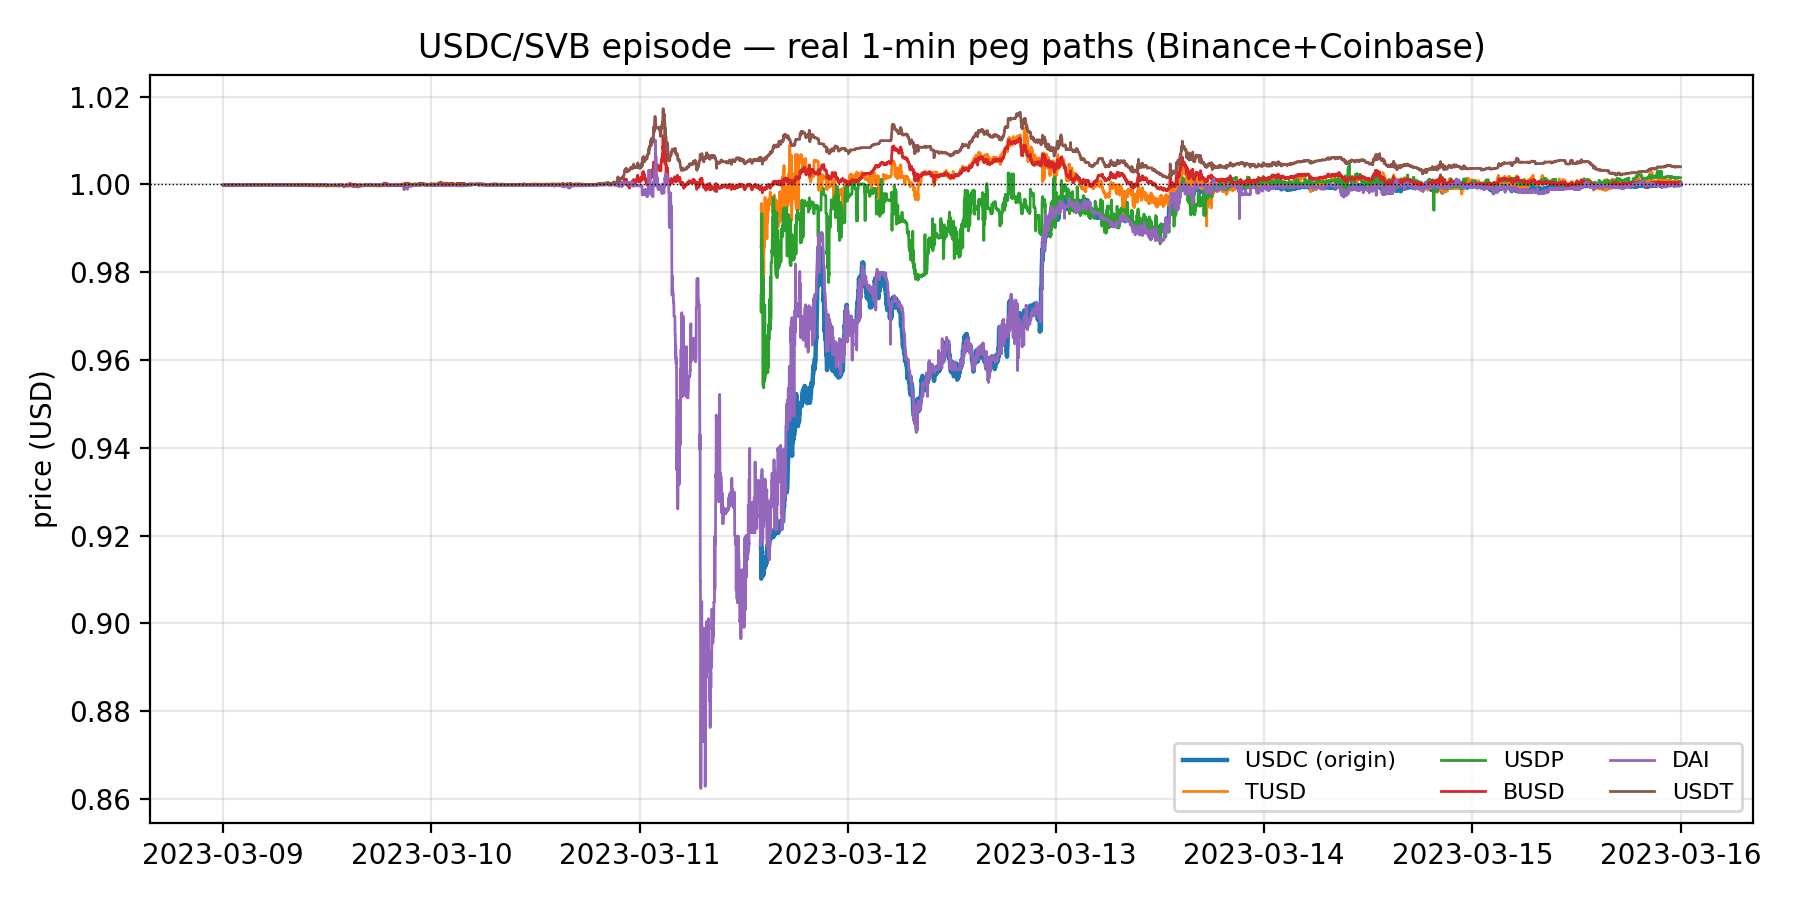
\includegraphics[width=\columnwidth]{figures/01_depeg_paths.png}
\caption{Real 1-minute peg paths during USDC/SVB (Binance + Coinbase): USDC and peers crash to
\$0.86--0.95 on 11 March 2023 and recover by the 13th.}
\label{fig:depeg}
\end{figure}

\section{Part I: Predicting Contagion (GNN)}
We run a model ladder---majority, persistence, logistic regression,
XGBoost~\cite{chen2016xgboost}, a GRU, GraphSAGE~\cite{hamilton2017graphsage}, and
GAT~\cite{velickovic2018gat}---on identical samples, with a leakage-safe held-out SVB cluster and
leave-one-cluster-out (LOCO).

\paragraph{Lead-time.} Contagion onset is unpredictable at horizons $\le 4$h (every model
$\approx$ base rate) but predictable at \textbf{24h}. Because PR-AUC rises mechanically with the
base rate, we report ROC-AUC (base-rate-free) and PR-AUC \emph{lift}; at 24h only the graph
models clear ROC-AUC $0.5$ and positive lift, GraphSAGE reaching ROC $0.65$
(Fig.~\ref{fig:leadtime}).

\begin{figure}[t]
\centering
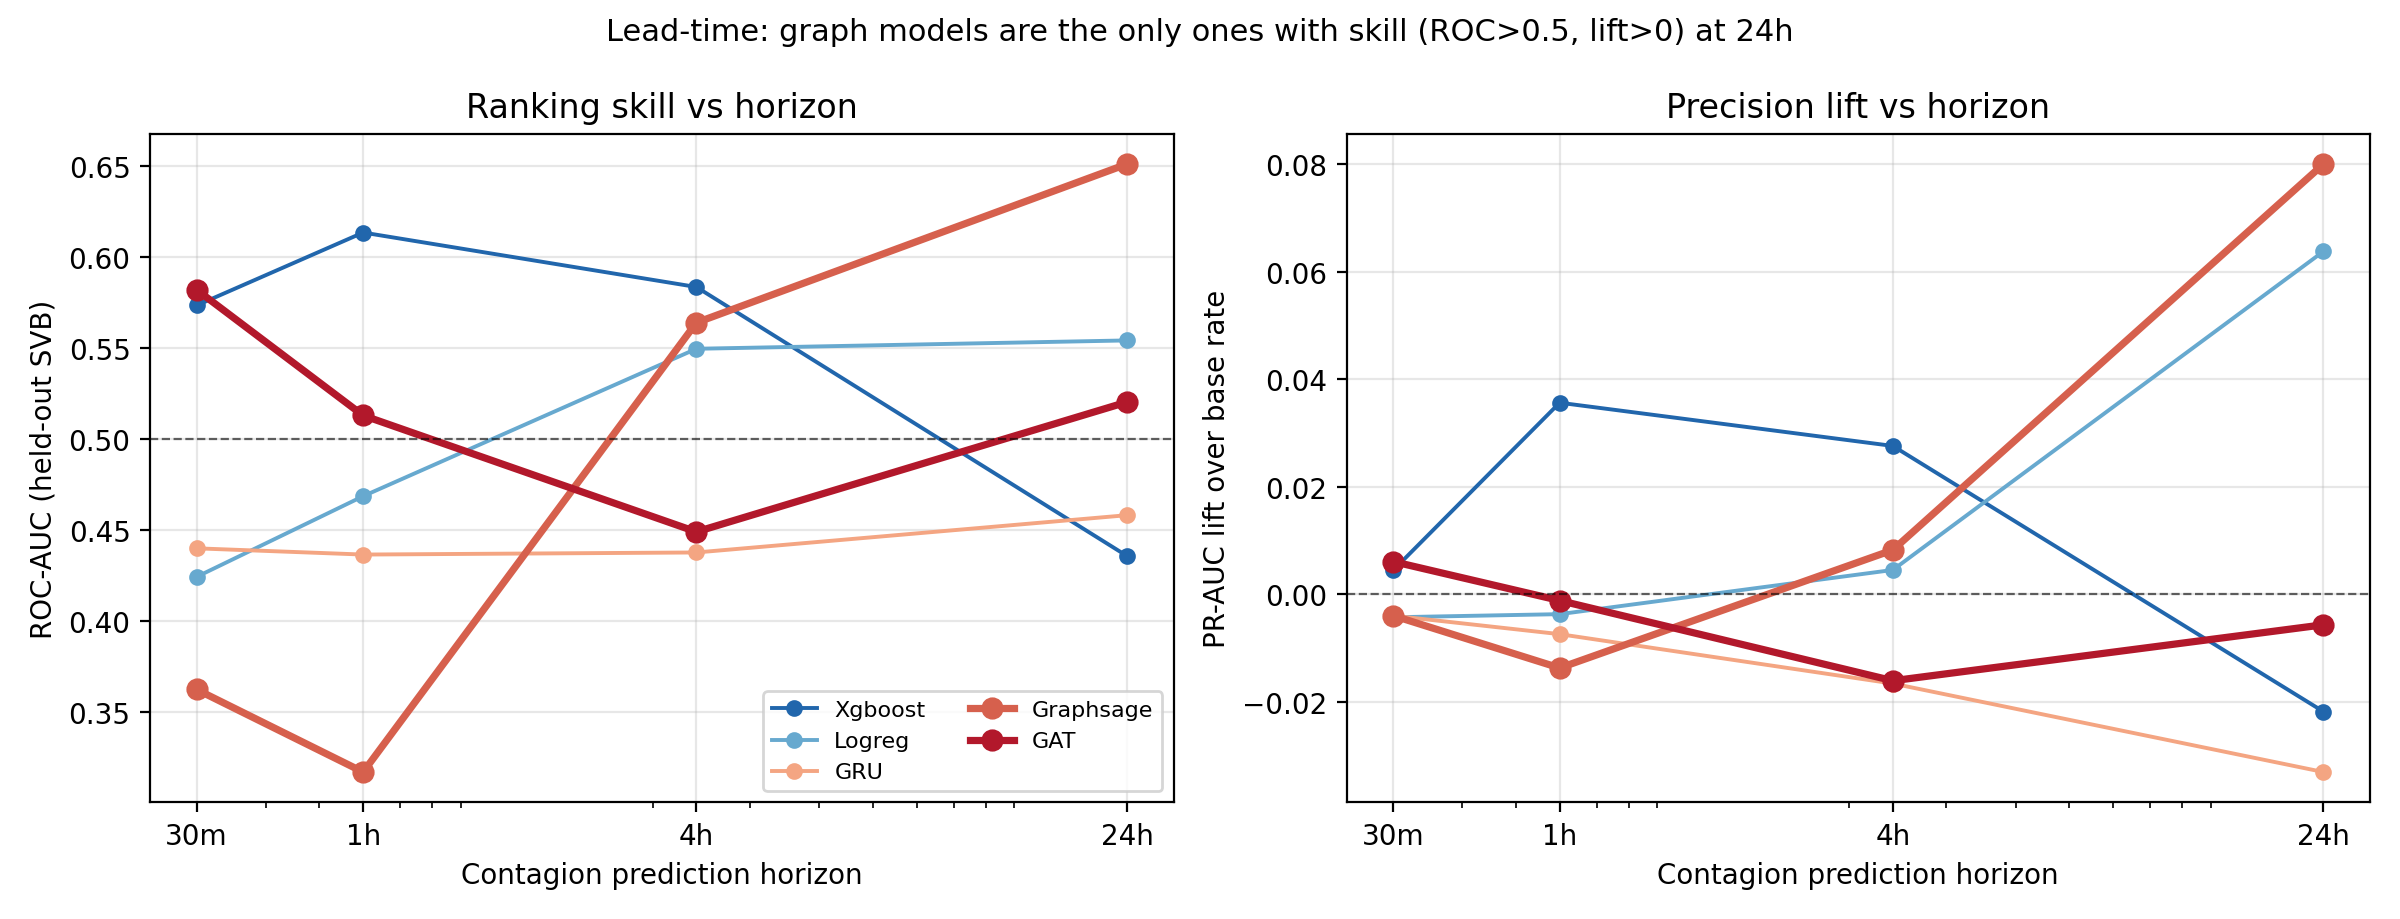
\includegraphics[width=\columnwidth]{figures/02_leadtime.png}
\caption{Lead-time. Left: ROC-AUC vs horizon---only the graph models exceed $0.5$ at 24h. Right:
PR-AUC lift over the base rate. Per-node tabular models hug chance.}
\label{fig:leadtime}
\end{figure}

\paragraph{Headline (5 seeds).} On the held-out SVB cluster at 24h, GAT attains PR-AUC
$0.447\pm0.016$, a margin of $+0.175\pm0.016$ over XGBoost (which sits at the base rate $0.29$).
LOCO margins are smaller but positive (GAT $+0.08$ Terra, $+0.03$ FTX) and survive dropping the
single-positive USDT-2018 fold (GAT $+0.083$). Adding per-node GRU temporal memory (TGN-lite)
adds $+0.008$ mean LOCO PR-AUC over static GAT (2 seeds; consistent on FTX folds, inconsistent
elsewhere), confirming the rolling 6h edge graph already captures most temporal dynamics.

\paragraph{Ablation.} A four-condition ablation isolates each component's contribution
(Table~\ref{tab:ablation}). The directed lead-lag \textbf{edges add $+0.100$ PR-AUC for GAT}
but only $+0.009$ for GraphSAGE. A third condition---keeping edges but zeroing all node
features---shows GAT collapses to the base rate ($0.293$), confirming that topology and
microstructure are complementary: neither is sufficient alone.

\begin{table}[t]
\caption{Four-condition component ablation, held-out SVB @ 24h. Condition~3 (topology only,
features zeroed) confirms that edges and node features are complementary.}
\label{tab:ablation}
\begin{tabular}{lrr}
\toprule
Condition & PR-AUC & vs.\ XGBoost \\
\midrule
(1) node-only (XGBoost) & 0.271 & --- \\
(2) GAT, no edges & 0.347 & $+0.075$ \\
(3) GAT, topology only (feat. zeroed) & 0.293 & $\approx$base rate \\
(4) GAT, full & \textbf{0.447} & $\mathbf{+0.175}$ \\
\midrule
\multicolumn{2}{l}{\small edge contribution (4)$-$(2):} & $+0.100$ \\
\bottomrule
\end{tabular}
\end{table}

\paragraph{Hub ranking (the hand-off).} Top microstructure precursors (XGBoost gain) are the OU
half-life and 24h realized volatility. The hub ranking combines GNN occlusion-influence,
betweenness, and a non-circular propagator label computed from raw prices. For USDC/SVB it flags
\textbf{BUSD} as the \#1 hub (highest betweenness $0.071$ and GNN influence $12.3$;
Fig.~\ref{fig:hubmap})---the input to the causal test. Attention-weight analysis adds granularity:
the top-attended directed \emph{edge} is USDC/Binance\,$\to$\,TUSD/Binance ($\bar\alpha=0.51$,
$1.9\times$ network average), with USDC appearing in four of the top-ten edge pairs, confirming
it as the dominant source node despite BUSD topping the betweenness ranking.

\begin{figure}[t]
\centering
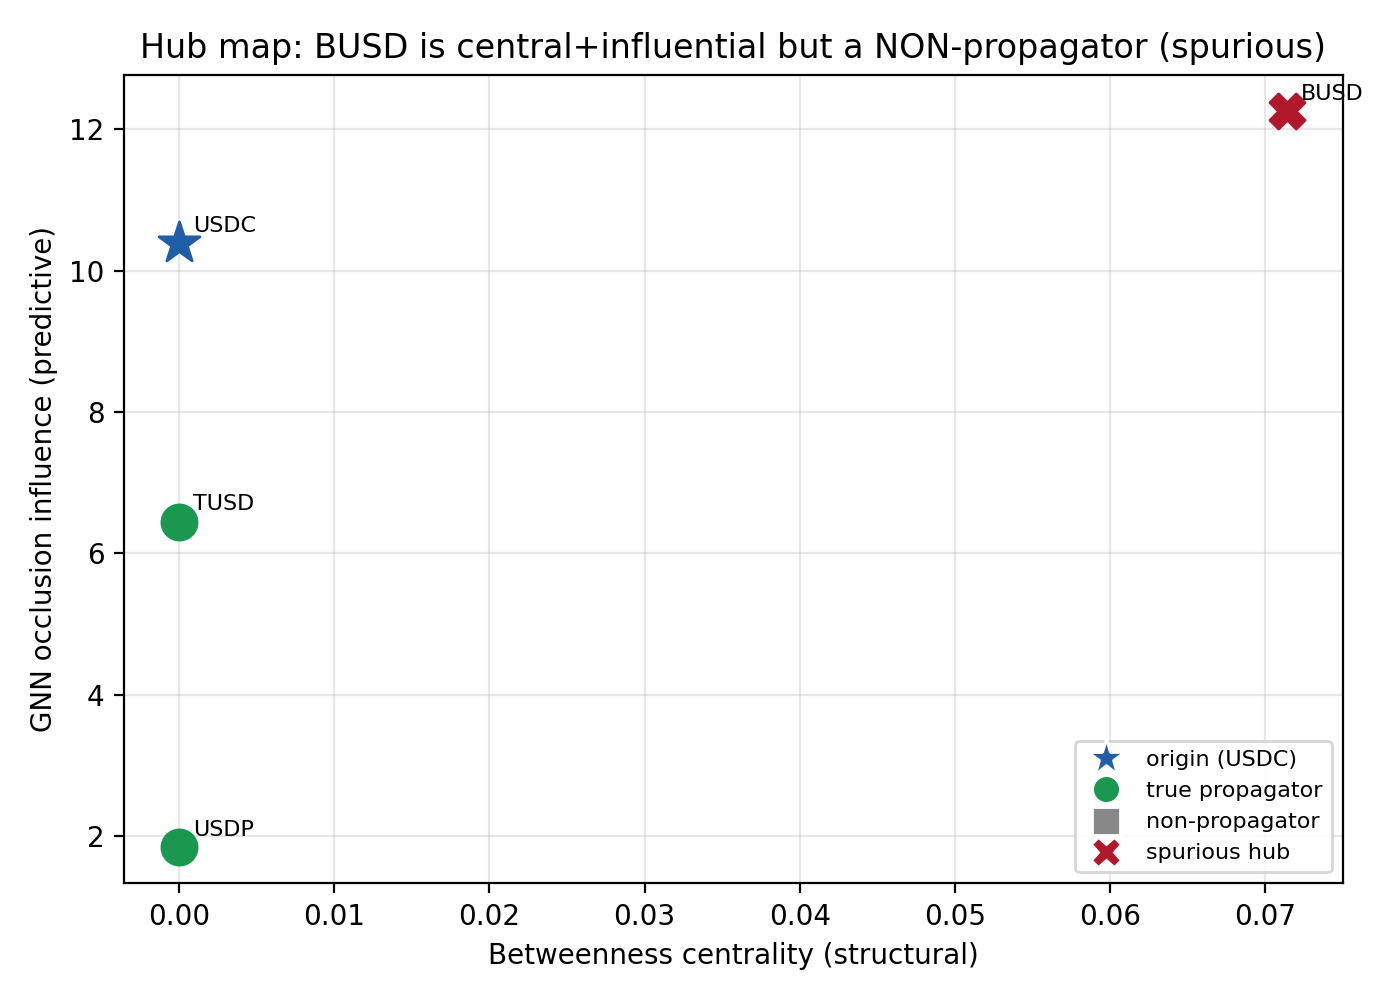
\includegraphics[width=\columnwidth]{figures/03_hub_map.png}
\caption{GNN hub map for USDC/SVB. BUSD has the highest centrality and influence yet is a
non-propagator (origin USDC marked separately).}
\label{fig:hubmap}
\end{figure}

\section{Part II: Causal Validation}
An AMM-only market is \emph{bimodal} (it resists a shock or collapses), so it cannot smoothly
reach a $\sim14\%$ depeg and fails the calibration gate. We use a \textbf{networked-contagion
model} in the spirit of network-propagation systemic-risk
measures~\cite{battiston2012debtrank}: per-asset near-critical mean-reverting peg dynamics with a
directed transmission matrix $W$ and an origin-driven panic channel,
\begin{equation}
d_i(t{+}1) = (1{-}\kappa)d_i(t) + c\!\sum_j W_{ij}\,\mathrm{stress}(d_j(t)) + s_i(t) + \pi|d_o(t)| + \varepsilon,
\end{equation}
where $\mathrm{stress}(d)=d$ if $|d|\ge\theta$ else $0$ and $o$ is the origin. It calibrates
$4/4$ to USDC/SVB (Table~\ref{tab:calib}).

\begin{table}[t]
\caption{Calibration to USDC/SVB empirical moments (targets exported from the GNN repo).}
\label{tab:calib}
\begin{tabular}{lrrc}
\toprule
moment & empirical & simulated & pass \\
\midrule
contagion magnitude & 0.1376 & 0.1376 & \checkmark \\
crisis half-life (steps) & 116 & 116.0 & \checkmark \\
baseline price vol & 0.0030 & 0.0029 & \checkmark \\
cross-venue $\rho$ & 0.576 & 0.640 & \checkmark \\
\bottomrule
\end{tabular}
\end{table}

\paragraph{Causal knockout.} Protecting a node (holding it at peg) and measuring the change in
contagion to the \emph{other} victims (deterministic propagation, fixed measure set) isolates its
causal effect. Protecting the origin USDC removes $100\%$ of contagion (a sanity check the model
passes). \textbf{BUSD's causal $\Delta = 0$} with out-transmission $0$: the GNN's \#1 hub is
causally inert. The Spearman correlation between GNN predicted importance and ABM causal effect
is $-0.77$ (Fig.~\ref{fig:join}).

\begin{figure}[t]
\centering
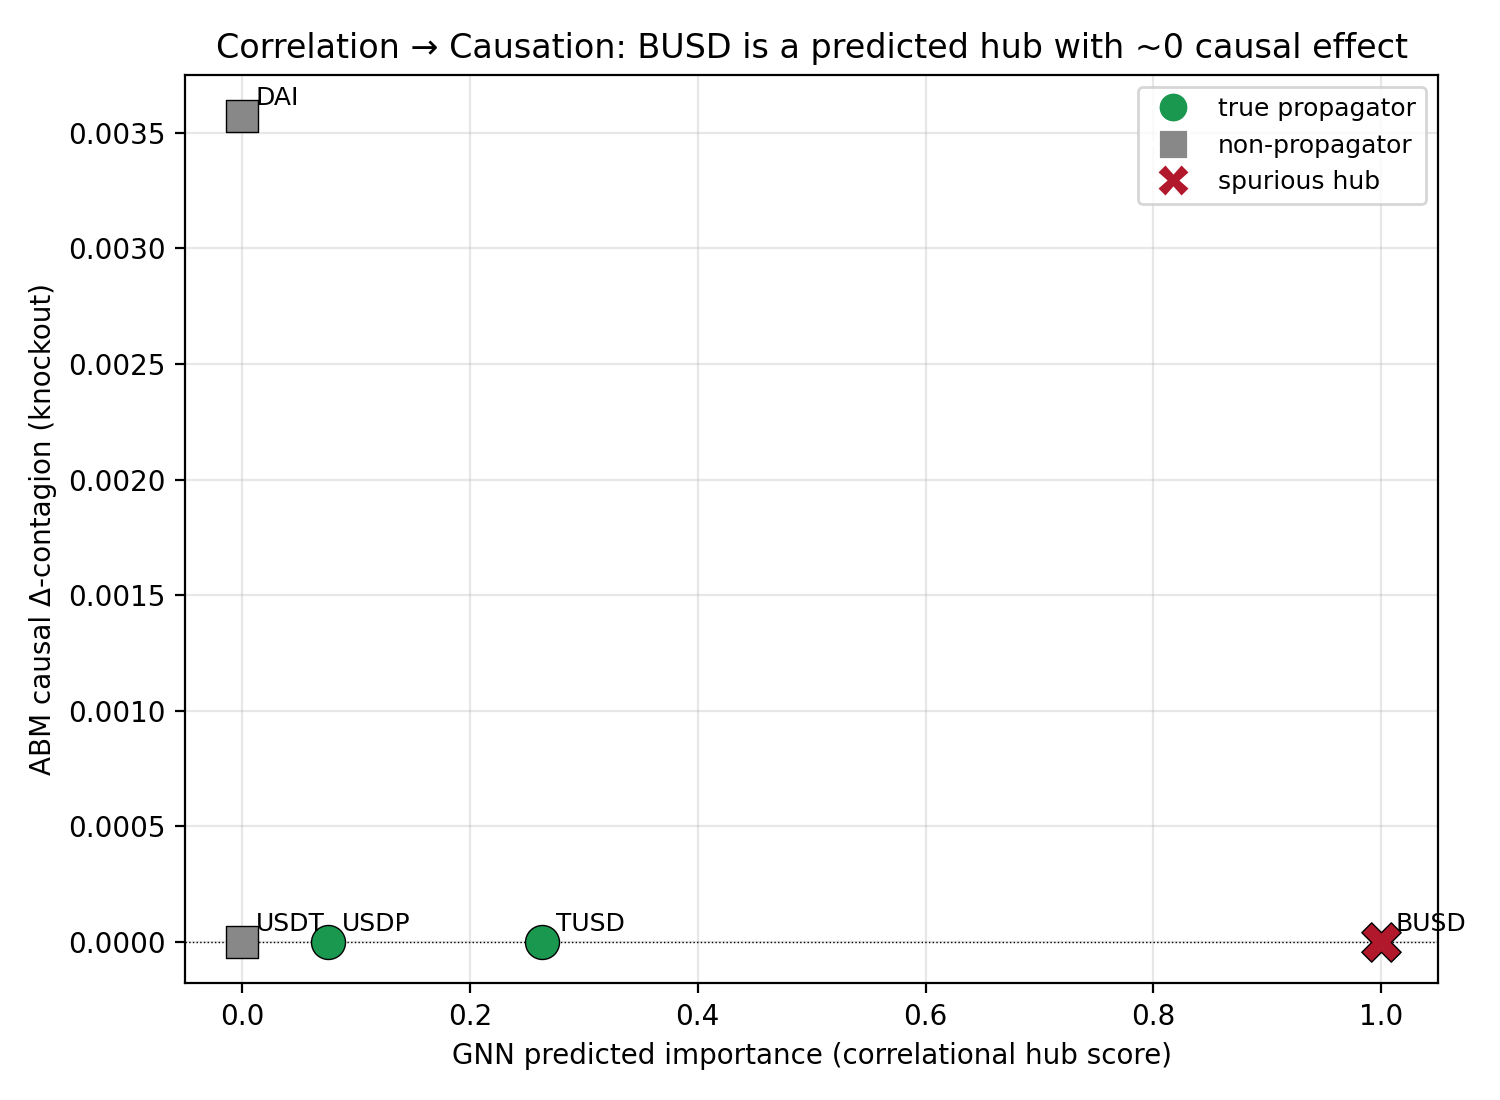
\includegraphics[width=\columnwidth]{figures/04_causal_join.png}
\caption{Correlation $\to$ causation. BUSD (the GNN's \#1 predicted hub) has causal
$\Delta\approx 0$; the actual relay (DAI) was not flagged.}
\label{fig:join}
\end{figure}

\paragraph{Why BUSD is spurious: balance sheets.} To remove any worry that the transmission
network is itself estimated from the same prices, we rebuild $W$ from \emph{documented} reserve
exposures: DAI and FRAX held USDC ($\sim$50\% and $\sim$90\%) during the window, while BUSD,
TUSD, USDP, and USDT held no other stablecoin and---critically---\emph{no stablecoin held BUSD as
backing}. Under this network the model still calibrates $4/4$, and BUSD's documented out-exposure
is $0.00$ (Fig.~\ref{fig:exposure}): it is \emph{mechanically} incapable of transmitting. The
exposure-based and lead-lag-based causal rankings agree (BUSD inert, origin dominant under both),
so the finding does not depend on how the structure is derived.

\begin{figure}[t]
\centering
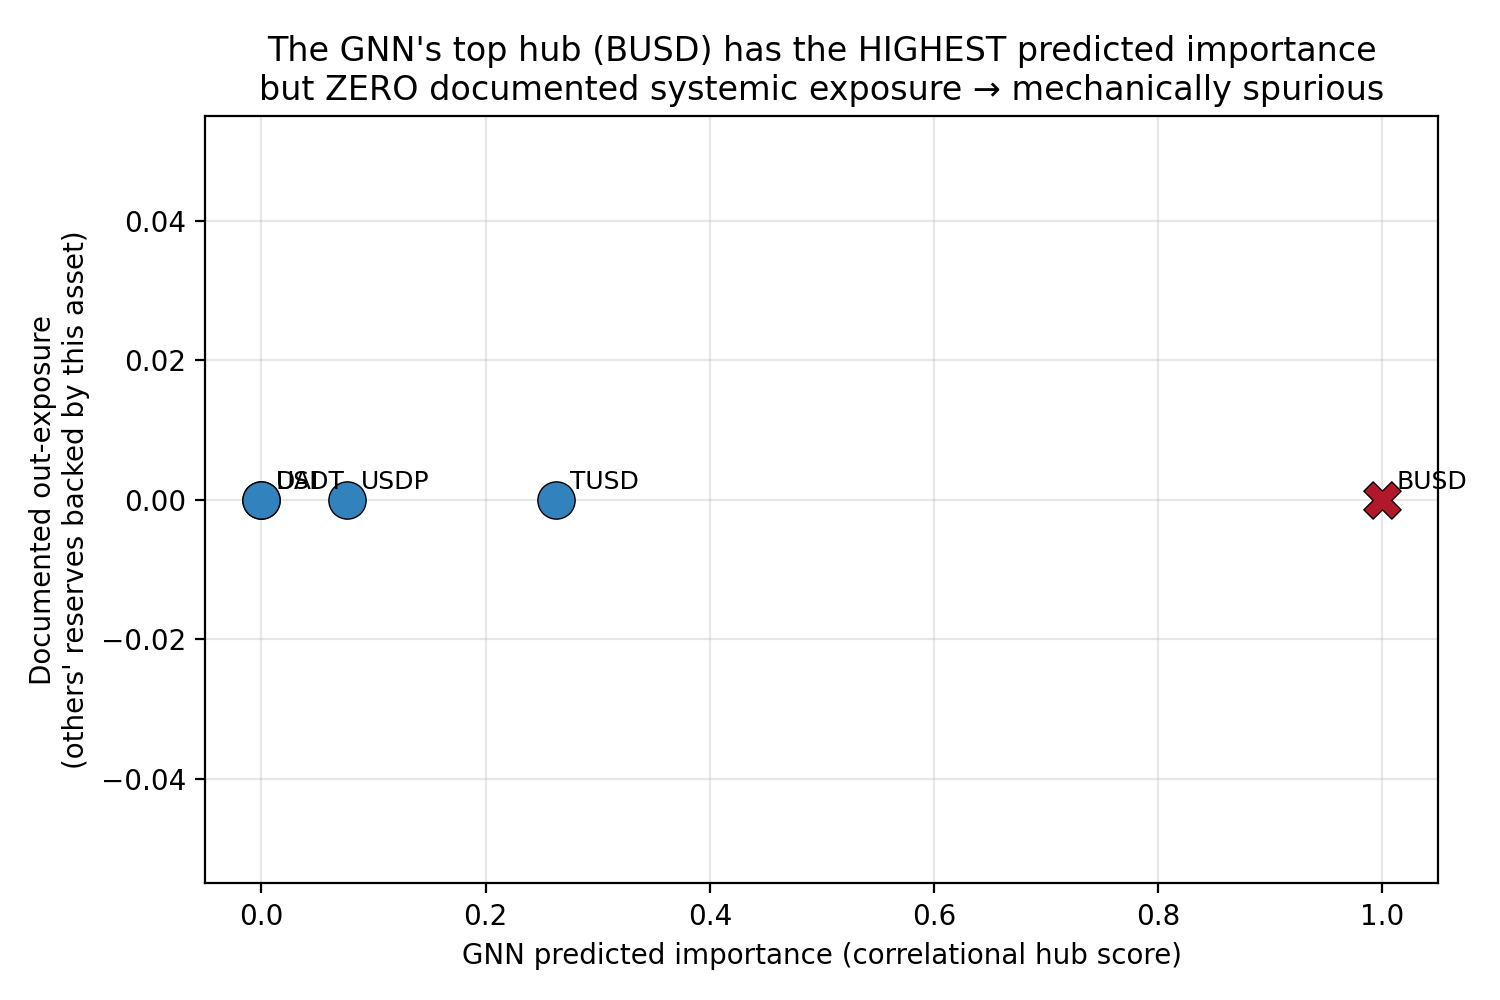
\includegraphics[width=\columnwidth]{figures/05_exposure.png}
\caption{The GNN's top hub (BUSD) has the highest predicted importance but \emph{zero} documented
systemic exposure---no stablecoin's peg depends on it.}
\label{fig:exposure}
\end{figure}

\section{Robustness}
Four independent checks. (1) \textbf{Calibration uncertainty}: under $\pm30\%$ perturbation of
$(c,\kappa,W)$ over 60 draws, USDC is the top causal node $100\%$ of the time and BUSD stays inert
$100\%$. (2) \textbf{Strategic agents}: we add an endogenous adaptive redeemer (redemptions accelerate
past a threshold, destabilising) and a capital-capped arbitrageur (a peg-restoring force subject
to limits-to-arbitrage, stabilising). The redeemer amplifies contagion $7.7\times$ and the
arbitrageur damps it, but across all four agent configurations the origin stays the top causal
node and BUSD stays inert---a Lucas-critique check the conclusions pass. Notably the
\emph{intervention} ranking flips: a circuit breaker overtakes reserve-strengthening ($95\%$ vs
$30\%$) once runs are self-reinforcing, so static-agent analysis would mis-rank policies. (3) \textbf{Structure derivation}: exposure-based
and lead-lag-based networks agree on the marquee result. (4) \textbf{Placebo control}: on
synthetic data with known ground truth, the knockout assigns causal $\Delta=0.139$ to true
transmitters and \emph{exactly zero} to a planted spurious co-mover that correlation centrality
cannot distinguish (Fig.~\ref{fig:placebo}).

\begin{figure}[t]
\centering
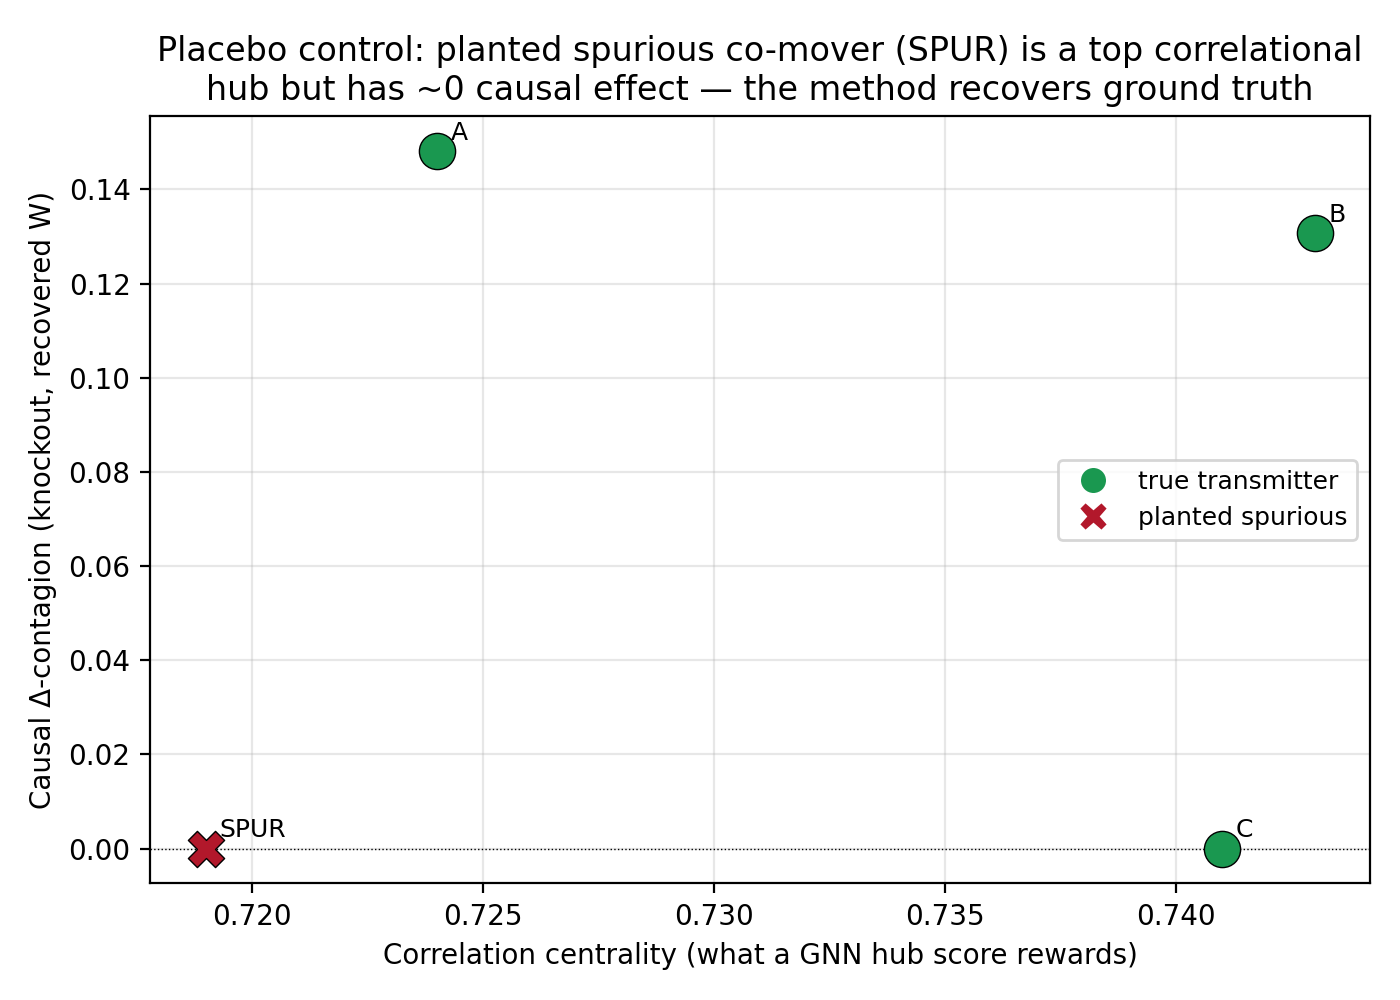
\includegraphics[width=\columnwidth]{figures/07_placebo.png}
\caption{Placebo control. A planted spurious co-mover (SPUR) is correlationally central but
causally inert; the method recovers ground truth.}
\label{fig:placebo}
\end{figure}

\paragraph{Generalization.} Across the three contagion-producing episodes the GNN's top hub
\emph{equals} the causal driver once (Terra) but \emph{diverges} twice (SVB, USDT-May), so
correlational rankings are unreliable and the causal test is necessary. A static, documented
quantity---out-exposure---ranks causal importance better than the learned GNN score (Spearman
$0.20$ vs $0.09$), and the GNN's top hub is a zero-exposure (structurally non-transmitting) node
in $3/5$ episodes.

\section{Part III: Policy}
Targeted protection of USDC cuts contagion $100\%$; reserve-strengthening USDC $\times20$ cuts
$89\%$; a circuit breaker $85\%$; redemption gating $100\%$. Protecting or strengthening BUSD cuts
$0\%$ at every intensity. The budget result is stark (Fig.~\ref{fig:interventions}): a regulator
who backstops one venue by the GNN's correlational ranking protects BUSD ($0\%$ reduction); by the
causal ranking protects USDC ($100\%$). A PPO regulator given only transmission-network features
(no causal labels) learns to allocate its reserve budget USDC $1.0$ / DAI $0.48$ / \textbf{BUSD
$0.0$}, achieving $93.7\%$ reduction---independently rediscovering the causal targets and ignoring
the spurious hub.

\begin{figure}[t]
\centering
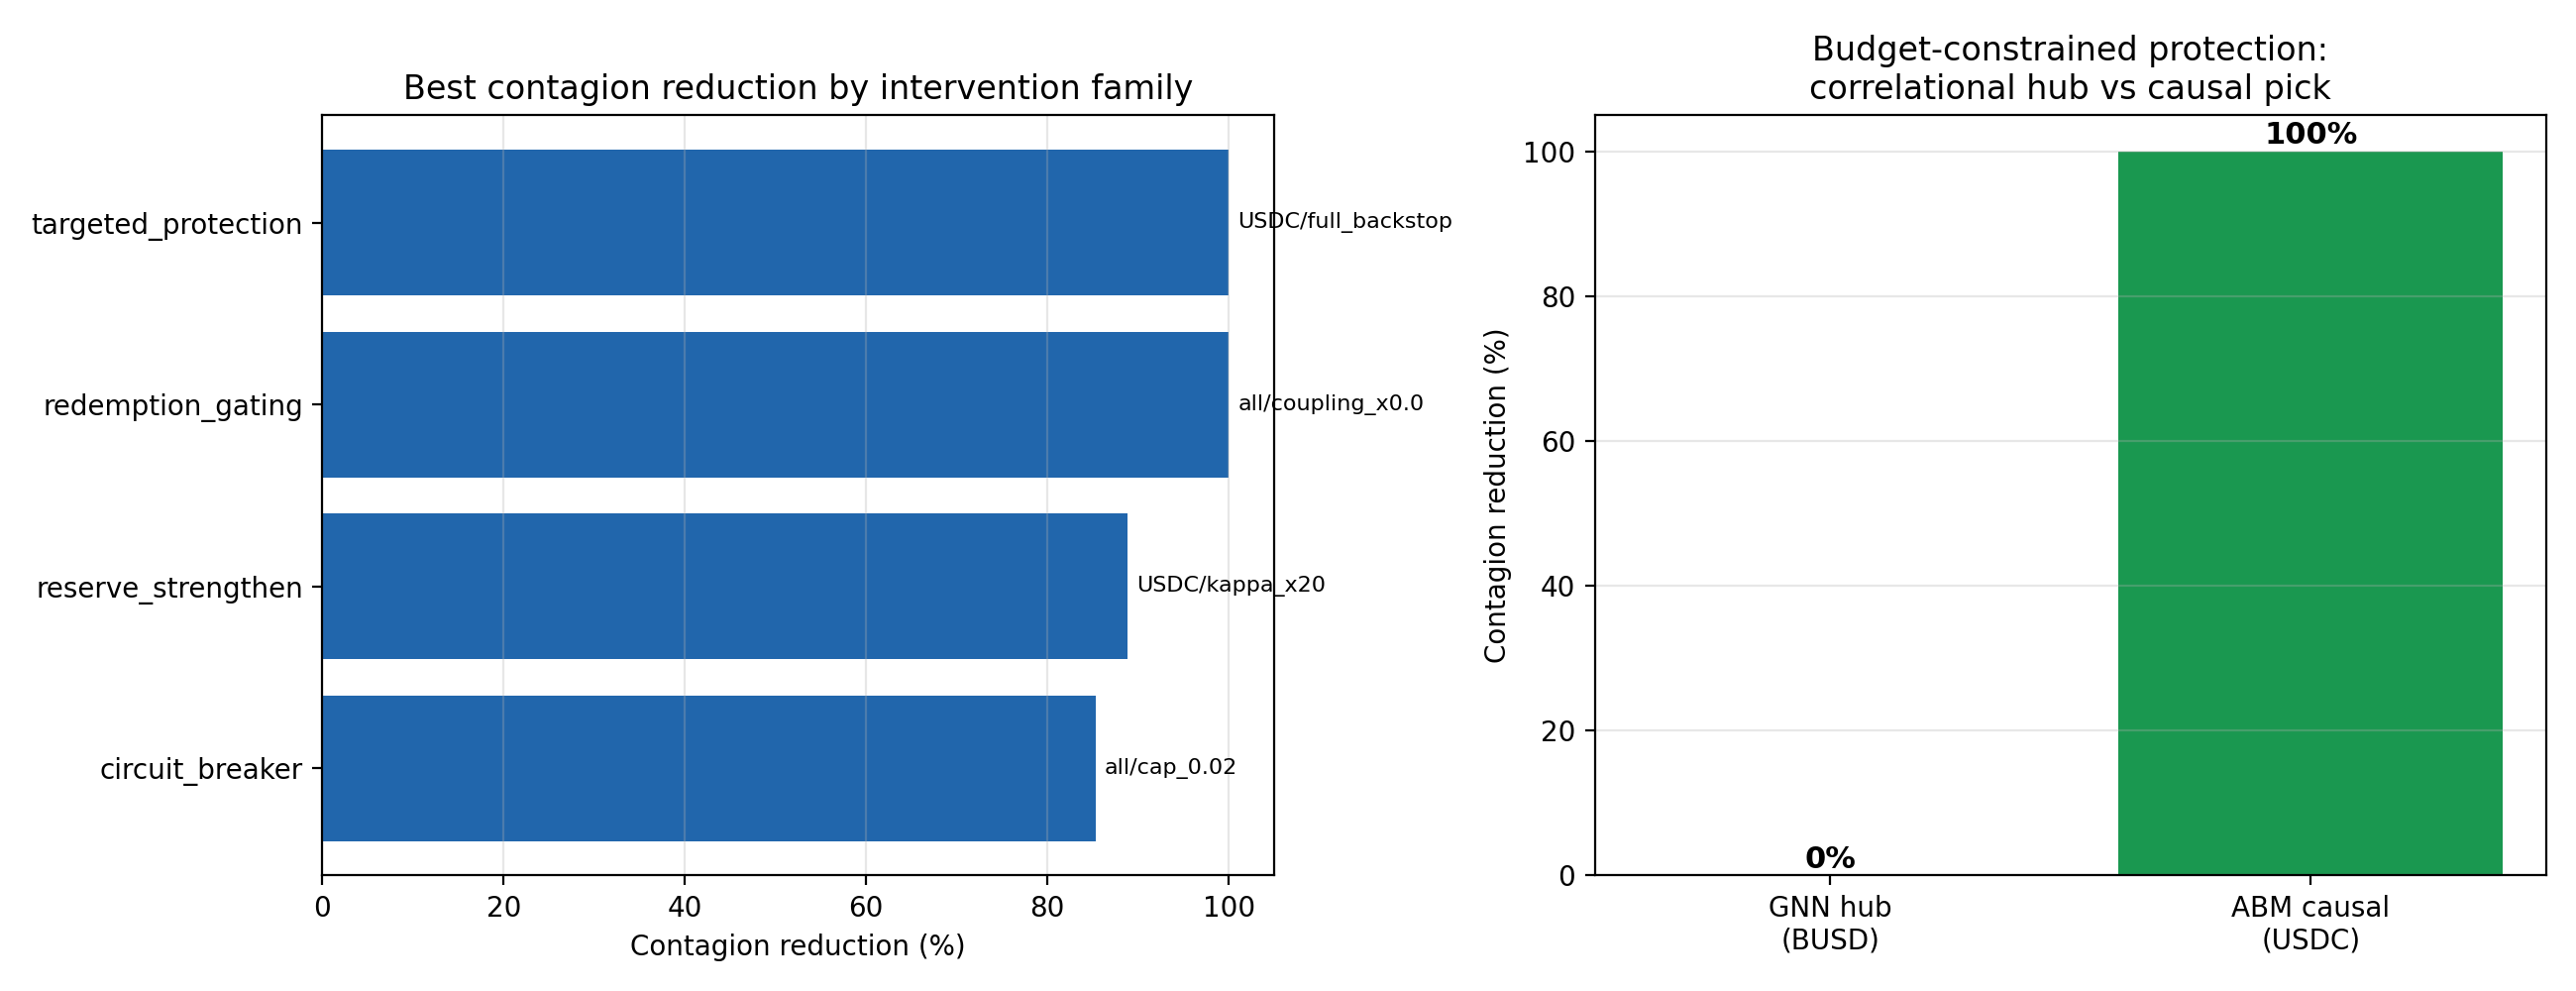
\includegraphics[width=\columnwidth]{figures/06_interventions.png}
\caption{Left: best contagion reduction by intervention family. Right: a one-venue budget spent on
the GNN's correlational hub (BUSD) yields $0\%$; on the causal pick (USDC), $100\%$.}
\label{fig:interventions}
\end{figure}

\section{Limitations}
$n=7$ episodes; two are too thin ($1$--$3$ active nodes, $\sim0$ contagion) to analyse causally.
The lead-lag $W$ can over-credit thinly traded coins as ``leaders,'' so the load-bearing claim is
the BUSD divergence---confirmed by the independent balance-sheet derivation. The networked model
is a reduced form for the causal analysis; short-horizon contagion is genuinely unpredictable
here, an honest negative that scopes the prediction claim.

\section{Conclusion}
A GNN can predict day-scale stablecoin contagion, and graph attention adds real signal---but its
hub rankings are correlational, and in the marquee SVB crisis its top hub (BUSD) causes \emph{no}
contagion because no stablecoin's peg depends on it. A calibrated, balance-sheet-grounded
contagion model supplies the missing causal test, and the disagreement matters: acting on the
correlational hub wastes the entire intervention budget the causal target would have spent to
contain the cascade. For reserve-transparency and intervention design under the GENIUS Act and
MiCA, contagion analytics should report \emph{causation}, validated---not correlation alone.

\paragraph{Reproducibility.} All numbers come from committed, scripted runs in the two
repositories; each repo's \texttt{reproduce.sh} regenerates every result and figure end-to-end
(see also \texttt{RESULTS.md}).

\bibliographystyle{ACM-Reference-Format}
\bibliography{references}

\end{document}
